\subsection{Beschreibung HMI - Datenbank}
\label{kap:ClientGraphProgrammDatenbank}
Während des Aufzeichnens von Sensorwerten erfolgt das Abspeichern in eine Datenbank. Diese beinhaltet die Daten für jeden Sensor einzeln mit den Werten Beschleunigungswerten in x, y und z, sowie einen Zeitstempel. Die Datenbank kann durch das Betätigen des Buttons \textit{Show Database}, in der Hauptansicht des Programms, angezeigt werden (s. Abbildung \ref{fig:clientgraphdatabase}). Durch das Betätigen des Up-Down-Selectors erfolgt die AUswahl des entsprechenden Sensors.

\begin{figure}[H]
\centering
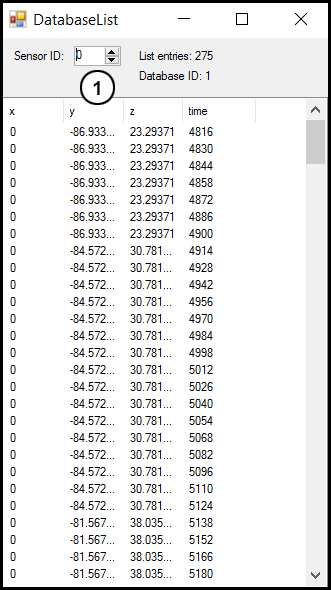
\includegraphics[width=0.5\linewidth]{Bilder/ClientGraphDatabase}
\caption[Datenbank mit Sensorwerten]{Datenbank mit Sensorwerten}
\label{fig:clientgraphdatabase}
\end{figure}
